\documentclass{article}
\usepackage{algorithm}
\usepackage{algpseudocode}
\usepackage{amsmath,amssymb,amsthm}
\usepackage{graphicx}
\usepackage[margin=1in]{geometry}
\usepackage{fancyhdr}
\usepackage{float}
\usepackage{longtable}
\setlength{\parindent}{0pt}
\setlength{\parskip}{5pt plus 1pt}
\setlength{\headheight}{13.6pt}
\newcommand\question[2]{\vspace{.25in}\hrule\textbf{#1: #2}\hrule\vspace{.10in}}
\renewcommand\part[1]{\vspace{.10in}\textbf{(#1)}}
\newcommand\algo{\vspace{.10in}\textbf{Algorithm: }}
\newcommand\correctness{\vspace{.10in}\textbf{Correctness: }}
\newcommand\runtime{\vspace{.10in}\textbf{Running time: }}
\newcommand\pseudoCode{\vspace{.10in}\textbf{PseudoCode: }}
\newcommand*{\perm}[2]{{}^{#1}\!P_{#2}}
\newcommand*{\comb}[2]{{}^{#1}\!C_{#2}}
%\pagestyle{fancyplain}
%\lhead{\textbf{\NAME\ (\UID)}}
%\chead{\textbf{Hw\HWNUM}}
%\rhead{CS 6350, \today}
\title{CS6350 - Homework/Assignment-6}
\author{Arnab Das(u1014840)}
\usepackage[utf8]{inputenc}
\begin{document}
  \pagenumbering{gobble}
  \maketitle
  \newpage
  \pagenumbering{arabic}
  \newcommand\NAME{ARNAB DAS}
  \newcommand\UID{uxxxxxxx}
  \newcommand\HWNUM{4}

  \question{1}{Warmup: Probabilities}
  \part{1} Given \newline
  \[ P(A_1) = P(A_2) = P(A_1 | A_2) = \dfrac{1}{2} \]

  From conditional probability:
  \[ P(A_1 , A_2) = P(A_1 | P(A_2))P(A_2) = \dfrac{1}{2} \times \dfrac{1}{2} = \dfrac{1}{4} \]

  Also, if we calculate the product of their individual probabilities :
  \[ P(A_1)P(A_2) = \dfrac{1}{2} \times \dfrac{1}{2} = \dfrac{1}{4} \]

  Hence, from the above two formulations, we have:
  \[ P(A_1 , A_2) = P(A_1 | P(A_2))P(A_2) = \dfrac{1}{2} \times \dfrac{1}{2} = \dfrac{1}{4} = P(A_1)P(A_2)\]

  Thus, $A_1, A_2$ are independent

  \part{2} Given, $A_1,A_2,A_3$ are mutually exclusive, $P(A_i) = \dfrac{1}{3}$ and $P(A_4 | A_i) = \dfrac{i}{6}$ . Then, we have the following probabilities: \newline
  \[P(A_1) = P(A_2) = P(A_3) = P(A_4) = \dfrac{1}{3}\]
  \[P(A_4|A_{i=1}) = \dfrac{1}{6}\]
  \[P(A_4|A_{i=2}) = \dfrac{1}{3}\]
  \[P(A_4|A_{i=3}) = \dfrac{1}{2}\]
  Using total probability theorem to evaluate $P(A_4)$, 
  \[ P(A_4) = P(A_1)P(A_4|A_1) + P(A_2)P(A_4|A_2) + P(A_3)P(A_4|A_3) \]
  \[ P(A_4) = \dfrac{1}{3}\times \dfrac{1}{6} + \dfrac{1}{3} \times \dfrac{1}{3} + \dfrac{1}{3}\times \dfrac{1}{2} = \dfrac{1}{3}\]

  \part{3} 
  Let n be the number at the top when a fair six-sided die is tossed. If a fair coin is tossed n times, required to find the probability of exactly two heads. \newline

  Now, we can get two heads only if the toss of the dice gives a number greater than equal to 2. For a single toss of an unbiased coin, we have the probabilites, $P(H) = \dfrac{1}{2}$ and $P(T) = \dfrac{1}{2}$ . Our problem is conditioned on the value of n that we get from the dice. So, we can write the probability of number of heads being exactly 2 as:
  \[P(H=2) = \sum_{n=2}^6P(H=2|n)P(n) \]
  $P(H=2) = P(H=2|n=2)P(n=2) + P(H=2|n=3)P(n=3) + P(H=2|n=4)P(n=4)$ \newline $ + P(H=2|n=5)P(n=5 ) + P(H=2|n=6)P(n=6)$

  Now for a specific n, $n \geq 2 $, the probability of exactly two heads = $\binom{n}{2} P(H)^2P(T)^{n-2}$ = $\binom{n}{2}\bigg (\dfrac{1}{2} \bigg )^2 \bigg ( \dfrac{1}{2} \bigg)^{n-2} = \binom{n}{2}\bigg ( \dfrac{1}{2} \bigg)^n$

  Also, since the we are given an unbiased fair dice, hence the probabilitities of getting a value of n between 1 to 6 will be equally probable, Hence, 
  \[ P(n=2) = P(n=3) = P(n=4) = P(n=5) = P(n=6) = \dfrac{1}{6} \]
  Using this formulation, in the expression for finding the probability of exactly two heads , we get:
  \[P(H=2) = \binom{2}{2}\bigg ( \dfrac{1}{2} \bigg )^2\dfrac{1}{6} + \binom{3}{2}\bigg ( \dfrac{1}{2} \bigg )^3\dfrac{1}{6} + \binom{4}{2}\bigg ( \dfrac{1}{2} \bigg )^4\dfrac{1}{6} + \binom{5}{2}\bigg ( \dfrac{1}{2} \bigg )^5\dfrac{1}{6} + \binom{6}{2}\bigg ( \dfrac{1}{2} \bigg )^6\dfrac{1}{6}\]

  \[P(H=2) = \bigg ( \dfrac{1}{2} \bigg )^2\dfrac{1}{6} + 3\bigg ( \dfrac{1}{2} \bigg )^3\dfrac{1}{6} + 6\bigg ( \dfrac{1}{2} \bigg )^4\dfrac{1}{6} + 10\bigg ( \dfrac{1}{2} \bigg )^5\dfrac{1}{6} + 15\bigg ( \dfrac{1}{2} \bigg )^6\dfrac{1}{6}\]

  \[P(H=2) = \dfrac{1}{6} \bigg (\bigg ( \dfrac{1}{2} \bigg )^2 + 3\bigg ( \dfrac{1}{2} \bigg )^3 + 6\bigg ( \dfrac{1}{2} \bigg )^4 + 10\bigg ( \dfrac{1}{2} \bigg )^5 + 15\bigg ( \dfrac{1}{2} \bigg )^6 \bigg ) = \dfrac{33}{128}\]

  \part{4} 
  Given $P(A_1) = a_1$ and $P(A_2) = a_2$. From conditional probability, we can write: 
  \[P(A_1 | A_2) = \dfrac{P(A_1 \cap A_2)}{P(A_2)} = \dfrac{P(A_1) + P(A_2) - P(A_1 \cup A_2)}{P(A_2)} \]

  Now, $P(A_1 \cup A_2) \leq 1$. Thus we get,
  \[P(A_1 | A_2) = \dfrac{P(A_1) + P(A_2) - P(A_1 \cup A_2)}{P(A_2)} \leq \dfrac{P(A_1) + P(A_2) - 1}{P(A_2)} \]
  replacing the given values of the probabilities, we get: \newline
  \[P(A_1 | A_2) = \dfrac{P(A_1) + P(A_2) - P(A_1 \cup A_2)}{P(A_2)} \leq \dfrac{a_1 + a_2 - 1}{a_2} \]


  \part{5a} If $A_1$ and $A_2$ are independent variables, show that: $E[A_1 + A_2] = E[A_1] + E[A_2]$ \newline
  \textbf{Proof:} Assuming $A_1$ and $A_2$ being independent discrete random variables, although the same holds for the continuous case.
  Then the expectation of $A_1$ is written as:
  \[E[A_1] = \sum_{a_1} a_1P(A_1 = a_1)\]
  where $a_1$ represents the values that $A_1$ can take and $P(a_2)$ represents their probabilities. Similarly,
  \[E[A_2] = \sum_{a_2} a_2P(A_2 = a_2) \]

  Then, we can write:
  \[E[A_1 + A_2] = \sum_{a_1} \sum_{a_2} (a_1 + a_2)P(A_1 = a_1, A_2 = a_2)\]
  or,
  \[E[A_1 + A_2] = \sum_{a_1} \sum_{a_2} a_1 P(A_1 = a_1, A_2 = a_2) + \sum_{a_1} \sum_{a_2} a_2 P(A_1 = a_1, A_2 = a_2)\]
  or,
  \[E[A_1 + A_2] = \sum_{a_1} a_1 \sum_{a_2} P(A_1 = a_1, A_2 = a_2) + \sum_{a_2} a_2 \sum_{a_1} P(A_1 = a_1, A_2 = a_2)\]

  Now, $\sum_{a_2}P(A_1 = a_1, A_2 = a_2) = P(A_1 = a_1)$, since we are summing over all the possible $a_2$ values that $A_2$ can take. Similarly, $\sum_{a_1}P(A_1 = a_1, A_2 = a_2) = P(A_2 = a_2)$. Plugging these back into the main equation, we get:
  \[E[A_1 + A_2] = \sum_{a_1} a_1 P(A_1 = a_1) + \sum_{a_2} a_2 P(A_2 = a_2) = E[A_1] + E[A_2]\]


  \part{5b} If $A_1$ and $A_2$ are independent variables, show that: $var[A_1 + A_2] = var[A_1] + var[A_2]$ \newline
  \textbf {Proof:} Variance of a random variable X is defined as:
  \[var(X) = E[(X - E[X])^2] = E[X^2 - 2XE[X] + (E[X])^2\]
  using the linearity of expectation as proved in the previous question, we can separate out the terms as:
  \[var(X) = E[X^2] - 2E[XE[X]] + E[(E[X])^2]\]
  Now, $E[X]$ is the theoretical mean of the distribution and hence a constant. ALso, the expectation of a constant terms is the term itself. Hence:
  \[var(X) = E[X^2] - 2E[X]E[X] + E[X]^2] = E[X^2] - (E[X])^2\]

  Thus, the variance of the given independent random variables, $A_1,A_2$ will be:
  \[var(A_1) = E[A_1^2] - (E[A_1])^2]\]
  \[var(A_2) = E[A_2^2] - (E[A_2])^2]\]

  Then the variance of the sum of the two independent variables will be:
  \[var[A_1 + A_2] = E[(A_1 + A_2)^2] - (E[A_1 + A_2])^2 = E[(A_1 + A_2)^2] - (E[A_1] + E[A_2])^2\]
  \[var[A_1 + A_2] = E[A_1^2] + E[A_2^2] +2E[A_1A_2] - (E[A_1])^2 - (E[A_2])^2 - 2E[A_1]E[A_2]\]
  \[var[A_1 + A_2] = (E[A_1^2] - (E[A_1])^2) + (E[A_2^2] - (E[A_2])^2) + 2E[A_1A_2] - 2E[A_1]E[A_2]\]
  \[var[A_1 + A_2] = var[A_1] + var[A_2] + 2E[A_1A_2] - 2E[A_1]E[A_2] \]
  \begin{equation}
  var[A_1 + A_2] = var[A_1] + var[A_2] + 2\sum_{a_1}\sum{a_2}a_1a_2P(A_1 = a_1,A_2 = a_2) - 2E[A_1]E[A_2]
	  \label{eq:varsum}
  \end{equation}

  In $\eqref{eq:varsum}$, since the random variables, $A_1,A_2$ are independent, so we have, $P(A_1=a_1, A_2=a_2) = P(A_1=a_1)P(A_2=a_2)$. Plcaing this back in the equation and separating out the sum with their corresponding variables we get: 
  \[var[A_1 + A_2] = var[A_1] + var[A_2] + 2\sum_{a_1}a_1P(A_1=a_1)\sum_{a_2}a_2P(A_2 = a_2) - 2E[A_1]E[A_2]\]
  \[var[A_1 + A_2] = var[A_1] + var[A_2] + 2E[A_1]E[A_2] - 2E[A_1]E[A_2]\]
  \[var[A_1 + A_2] = var[A_1] + var[A_2] \]

  \question{2}{Naive Bayes}
  \part{1.a} We are given the true distribution values. If we draw infinite data from this distribution, then the empirically evaluated probabilities will converge close to the true distribution according to the law of large numbers which suggests for infinitely drawn data the sampled mean and the theoretical mean converges. Hence, after seeing infinitely drawn data, the evaluated probabilities can be approximated to the true distribution, in which case we have:
  \[\hat{P}(x_1 = -1| y = -1) = 0.8\]
  \[\hat{P}(x_1 = 1| y = -1) = 0.2\]
  \[\hat{P}(x_1 = -1| y = 1) = 0.1\]
  \[\hat{P}(x_1 = 1| y = 1) = 0.9\]
  \[\hat{P}(y=1) = 0.9 \]
  \[\hat{P}(y=-1) = 0.1 \]

  \part{1.b} Using the above probability values, we evaluate the required probabilities of the given table as :
  \[\hat{P}(x_1 = -1, y = -1) = \hat{P}(x_1 = -1| y = -1)\hat{P}(y= -1) = 0.08\]
  \[\hat{P}(x_1 = 1, y = -1) = \hat{P}(x_1 = 1| y = -1)\hat{P}(y= -1) = 0.02\]
  \[\hat{P}(x_1 = -1, y = 1) = \hat{P}(x_1 = -1| y = 1)\hat{P}(y= 1) = 0.09\]
  \[\hat{P}(x_1 = 1, y = 1) = \hat{P}(x_1 = 1| y = 1)\hat{P}(y= 1) = 0.81\]

  Hence, the prediction will be : 
  \[y^\prime\bigg |_{x_1=-1} = argmax_y\hat{P}(x_1=-1,y) = +1\]
  \[y^\prime\bigg |_{x_1=+1} = argmax_y\hat{P}(x_1=-1,y) = +1\]

  Thus, the table will be :
\begin{longtable}{c|c|c|c}
	\caption{Probability Table-1: Input $x_1$, $\hat{P}(x_1,y=-1)$,$\hat{P}(x_1,y=1)$ ,Prediction: $y^\prime = arg max_y \hat{P}(x_1,y)$} \\
  %\centering
  %\begin{tabular}{c c c c}
  \hline\hline
	  Input $x_1$ & $\hat{P}(x_1,y=-1)$ & $\hat{P}(x_1,y=1)$  & Prediction: $y^\prime = arg max_y \hat{P}(x_1,y)$ \\ [0.5ex]
  \hline
	  -1 & 0.08 & 0.09 & +1  \\
	  +1 & 0.02 & 0.81 & +1 \\
  \end{longtable}


  \part{1.c} To find the error in predictions, we need to find $P(y^\prime \neq y)$, Thus:
  \[ P(y^\prime \neq y) = P(y^\prime \neq y, x_1 = -1) + P(y^\prime \neq y, x_1 = +1)\]
  $P(y^\prime \neq y) = P(y^\prime = 1,x_1 = -1)P(y=-1,x_1=-1) + P(y^\prime =-1,x_1 = -1)P(y=+1,x_1=-1)$ \newline
	$ + P(y^\prime = +1, x_1 = +1)P(y=-1, x_1 = +1) + P(y^\prime = -1, x_1 = +1)P(y=+1, x_1 = +1)$ \newline
  $P(y^\prime \neq y) = P(y^\prime = 1,y=-1,x_1 = -1) + P(y^\prime =-1,y=+1,x_1 = -1)$ \newline
	$ + P(y^\prime = +1,y=-1, x_1 = +1) + P(y^\prime = -1, x_1 = +1)P(y=+1, x_1 = +1)$ \newline
  $P(y^\prime \neq y) = 0.08 + 0 + 0.02 + 0 = 0.1 $


 \part{2.a} Given a binary classification problem with two features , $x_1,x_2$, both of which can take discrete values \{-1,1\}. Additionaly, the feature $x_2$, is exactly identical to first feature $x_1$. \newline
	Since, $x_1$ and $x_2$ are identical/same feature, hence:
	\[P(x_1 |y) = P(x_2|y)\]
	and, since $x_1$ and $x_2$ will have identical values under all conditions, hence\newline
	$P(x_1 = a_1 | x_2 = a_2) = 1$, if $a_1 = a_2$ \newline
	$P(x_1 = a_1 | x_2 = a_2) = 0$, if $a_1 \neq a_2$ \newline

	Now, from conditional probability, we can write:
	\[P(x_1,x_2 | y) = P(x_1 | x_2,y) P(x_2 | y)\]
	For condittional independence, we require,
	\begin{equation}
		P(x_1,x_2 | y) = P(x_1 | y) P(x_2|y)
		\label{eq:condInd}
	\end{equation}

	However, in this case, since $x_1$ and $x_2$, are the same feature, hence the probability of $x_1$, given $x_2$ and $y$, will be same as probability of $x_2$ given y, multiplied with the gating function $P(x_1 | x_2)$ which means $P(x_1 | x_2,y) = P(x_1 | x_2)$ such that if $x_1=x_2$, it is one, and if $x_1 \neq x_2$, it is zero. Thus, we have,
	\[P(x_1,x_2 | y) = P(x_1 | x_2,y) P(x_2 | y) = P(x_1 | x_2) P(x_2|y)\]
	This differs from the requirement of conditional independence in $\eqref{eq:condInd}$. Hence, $x_1$ and $x_2$ are \textbf {not} conditionally independent, given y. 

 \part{2.b}
	Given that $\hat{P}(x_1 | y)$, $\hat{P}(x_2 | y)$ and $\hat{P}(y)$ represent the learned parameters of a Naive Bayes(NB) classifier on infinite data set, so the values of these probabilities will be same as in the previous question. Hence,evaluating the probabilities in the table: \newline
	$1. \hat{P}(x_1 = -1,x_2 = -1,y = -1 )$ = $\hat{P}(x_1= -1| y=-1 )\hat{P}(x_2= -1| y= -1)\hat{P}(y= -1) = 0.8\times 0.8 \times 0.1 = 0.064$ \newline
	$2. \hat{P}(x_1 =-1 ,x_2 =1 ,y = -1 )$ = $\hat{P}(x_1=-1 | y=-1 )\hat{P}(x_2=1 | y= -1)\hat{P}(y= -1) = 0.8 \times 0.2 \times 0.1 = 0.016$ \newline
	$3. \hat{P}(x_1 = 1,x_2 =-1 ,y = -1 )$ = $\hat{P}(x_1=1 | y=-1 )\hat{P}(x_2=-1 | y= -1)\hat{P}(y= -1) = 0.2\times 0.8 \times 0.1 = 0.016$ \newline
	$4. \hat{P}(x_1 =1 ,x_2 =1 ,y = -1 )$ = $\hat{P}(x_1=1 | y=-1 )\hat{P}(x_2= 1| y= -1)\hat{P}(y= -1) = 0.2 \times 0.2 \times 0.1 = 0.004$ \newline

 
	$5. \hat{P}(x_1 = -1,x_2 = -1,y = 1 )$ = $\hat{P}(x_1= -1| y=1 )\hat{P}(x_2= -1| y= 1)\hat{P}(y= 1) = 0.1\times 0.1 \times 0.9 = 0.009$ \newline
	$6. \hat{P}(x_1 =-1 ,x_2 =1 ,y = 1 )$ = $\hat{P}(x_1=-1 | y=1 )\hat{P}(x_2=1 | y= 1)\hat{P}(y= 1) = 0.1 \times 0.9 \times 0.9 = 0.081$ \newline
	$7. \hat{P}(x_1 = 1,x_2 =-1 ,y = 1 )$ = $\hat{P}(x_1=1 | y=1 )\hat{P}(x_2=-1 | y= 1)\hat{P}(y= 1) = 0.9\times 0.1 \times 0.9 = 0.081$ \newline
	$8. \hat{P}(x_1 =1 ,x_2 =1 ,y = 1 )$ = $\hat{P}(x_1=1 | y=1 )\hat{P}(x_2= 1| y= 1)\hat{P}(y= 1) = 0.9 \times 0.9 \times 0.9 = 0.729$ \newline

	Hence, the predictions will be like: $y^\prime\bigg |_{x_1=-1,x_2=-1} = argmax_y\hat{P}(x_1=-1,x_2=-1,y) = -1$. Similarly, filling up the table:
 % \[y^\prime\bigg |_{x_1=-1,x_2=1} = argmax_y\hat{P}(x_1=-1,x_2=1,y) = 1\]
 % \[y^\prime\bigg |_{x_1=1,x_2=-1} = argmax_y\hat{P}(x_1=1,x_2=-1,y) = 1\]
 % \[y^\prime\bigg |_{x_1=1,x_2=1} = argmax_y\hat{P}(x_1=1,x_2=1,y) = 1\]
  Thus the table will be:
\begin{longtable}{c|c|c|c|c}
	\caption{Probability Table-1: Input $x_1$, $x_2$, $\hat{P}(x_1,x_2,y=-1)$,$\hat{P}(x_1,x_2,y=1)$ ,Prediction: $y^\prime = arg max_y \hat{P}(x_1,x_2,y)$} \\
  %\centering
  %\begin{tabular}{c c c c c}
  \hline\hline
	  Input $x_1$ & $x_2$ & $\hat{P}(x_1,x_2,y=-1)$ & $\hat{P}(x_1,x_2,y=1)$  & Prediction: $y^\prime = arg max_y \hat{P}(x_1,x_2,y)$ \\ [0.5ex]
  \hline
	  -1 & -1 & 0.064 & 0.009 & -1 \\
	  -1 & 1 & 0.016 & 0.081 & +1 \\
	  1 & -1 & 0.016 & 0.081 & +1 \\
	  1 & 1 & 0.004 & 0.729 & +1 \\
  \end{longtable}

  \part{2.c} To find the error in prediction, we need to find $P*y^\prime \neq y)$. Thus,
	\[P(y^\prime \neq y) = P(y^\prime \neq y, x_1 =-1 , x_2 =-1 ) + P(y^\prime \neq y, x_1 =-1 , x_2 =1 ) + P(y^\prime \neq y, x_1 =1 , x_2 =-1 ) + P(y^\prime \neq y, x_1 =1 , x_2 =1 )\]
	$P(y^\prime \neq y,x_1=-1,x_2=-1) = P(y^\prime = 1,y=-1,x_1=-1,x_2=-1) + P(y^\prime =-1,y=+1,x_1=-1,x_2=-1) = 0 + 0.009 = 0.009$ \newline
	$P(y^\prime \neq y,x_1=-1,x_2=+1) = P(y^\prime = 1,y=-1,x_1=-1,x_2=+1) + P(y^\prime =-1,y=+1,x_1=-1,x_2=+1) = 0.016 + 0 = 0.016 $ \newline
	$P(y^\prime \neq y,x_1=+1,x_2=-1) = P(y^\prime = 1,y=-1,x_1=+1,x_2=-1) + P(y^\prime =-1,y=+1,x_1=+1,x_2=-1) = 0.016 + 0 = 0.016$ \newline
	$P(y^\prime \neq y,x_1=+1,x_2=+1) = P(y^\prime = 1,y=-1,x_1=+1,x_2=+1) + P(y^\prime =-1,y=+1,x_1=+1,x_2=+1) = 0.004$ \newline

	Therefore,
	\[P(y^\prime \neq y) = 0.009 + 0.016 + 0.016 + 0.004 = 0.045\]


	\part{2.d} Since Naive Bayes(NB) considers the features to be conditionally independent, hence if there exists features duplicated or strongly correlated, NB will treat them independently and give both of them strong weights such that they have double influence. On the other hand, Logistic-Regression(LR) does not have any conditional independence requirement and hence it performs better in cases where features might be duplicated or strongly correlated, since its minimization algorithm will tend to compensate for the correlation of features.

	\question{3}{Naive Bayes and Linear Classifiers}
	Given inputs as d-dimensional feature vector , \textbf {x} = $(x_1,x_2,\dots , x_d)^T$, where each $x_j$ can be a real number. Classifier predicts 1 if:
	\[ P(y=1 | x) \geq P(y=0 | x) \]
	\[ \dfrac{P(y=1 | x)}{P(y=0 | x)} \geq 1 \]
	or equivalently:
	\[ \dfrac{P(x|y=1)P(y=1)}{P(x|y=0)P(y=0)} \geq 1\]
	By the Naive Bayes assumption of conditional independence of the features, we have $P(x|y) = \prod_{j=0}^d P(x_j|y)$. Then we have $\dfrac{P(y=1)}{P(y=0)}\prod_{j=0}^d \dfrac{P(x_j|y=1)}{P(x_j|y=0)} \geq 1$ for the \textbf {decision boundary}. Suppose each $P(x_j|y)$ is defined using a Gaussian probability density function(pdf), one for each value of $y$ and $j$ with mean $\mu_{j,y}$ and variance $\sigma^2$. Thus, we can use the pdf expression for $P(x_j|y)$, such that the mean for $y=1$ and a specific $j$ is denoted as $\mu_{j,y_1}$ and the mean for $y=0$ and a specific $j$ is denoted as $\mu_{j,y_0}$. Also, let us denote the prior probability of $P(y=1)$ as $p$. Then the prior probability of $P(y=0)$ is $(1-p)$.
 Hence, we can write out the decision boundary as:
	\[\dfrac{p}{1-p} \prod_{j=0}^d \dfrac{\dfrac{1}{\sqrt[2]{2\pi \sigma^2}}e^{-\dfrac{(x_j - \mu_{j,y_1})^2}{2\sigma^2}}}{\dfrac{1}{\sqrt[2]{2\pi \sigma^2}}e^{-\dfrac{(x_j - \mu_{j,y_0})^2}{2\sigma^2}}} \geq 1\]

	\[\dfrac{p}{1-p} \prod_{j=0}^d e^{\dfrac{1}{2\sigma^2}(\mu_{j,y_1} - \mu_{j,y_0})(2x_j - \mu_{j,y_0} - \mu_{j,y_1}} \geq 1\]
	Taking natural lo on both sides and rearranging the terms to separate out $x_j$, we get:
	\[\log(\dfrac{p}{1-p}) + \dfrac{1}{2\sigma^2}\sum_{j=0}^d (\mu_{j,y_1} - \mu_{j,y_0})(-\mu_{j,y_1} - \mu_{j,y_0}) + \dfrac{1}{2\sigma^2} \sum_{j=0}^d 2x_j (\mu_{j,y_1} - \mu_{j,y_0}) \geq 0\]
	The means of each of the distributions are specific to the distributions and constant with respect to $x_j$. Furthermore, it is given the variance is same for all the distribution, hence it is also a constant with respect to $x_j$. Thus, from the above expression we can separate out the constant term as the bias, such that we can write the following: \newline
	bias = b = $\log(\dfrac{p}{1-p}) - \dfrac{1}{2\sigma^2}\sum_{j=0}^d (\mu_{j,y_1}^2 - \mu_{j,y_0}^2)$ and \newline
	weights, $w_j = \dfrac{1}{\sigma^2}(\mu_{j,y_1} - \mu_{j,y_0})$. \newline
	hence, we get the decision boundary as:
	\[ b + \sum_{j=0}^d w_jx_j \geq 0\]

	Hence, our classifier is a linear classifier. 

	\question{4}{Experiment}
	Given minimization problem: $\min_{\mathbf{w}}\{ \sum_{i=1}^m \log(1 + \exp(-y_i\mathbf{w}^T\mathbf{x_i})) + \dfrac{1}{\sigma^2}\mathbf{w^Tw} \}$
	\part{1} To find the derivative of the function: $g(\mathbf{w}) = \log(1 + \exp(-y_i\mathbf{w^Tx_i}))$. For an n-dimensional vector, its gradient will have derivative components with respect to each feature,$w_j$, that will be:
	\[ \dfrac{\partial g(\mathbf{w})}{\partial w_j} = \dfrac{\exp(-y_i\mathbf{w^Tx_i})(-y_ix_{ij})}{1 + \exp(-y_i\mathbf{w^Tx_i})} = \dfrac{-y_ix_{ij}}{1 + \exp(y_i\mathbf{w^Tx_i})}\]
	Thus, the overall gradient vector will be:
	\[\nabla g(\mathbf{w}) = [\dfrac{\partial g}{\partial w_1},\dfrac{\partial g}{\partial w_2}, \dots, \dfrac{\partial g}{\partial w_n}] = \dfrac{-y_i\mathbf{x_i}}{1 + \exp(y_i\mathbf{w^Tx_i})}\]

	\part{2} Gradient update is the innermost step of SGD where a single example is treated as the entire dataset to compute the gradient. The objective function for a single example $(\mathbf{x_i},y_i)$, will be:
	\[ J(\mathbf{w}) = \log(1 + \exp(-y_i\mathbf{w^Tx_i})) + \dfrac{1}{\sigma^2}\mathbf{w^Tw} \]
	The partial derivative with respect to weight component $w_j$ will be:
	\[ \dfrac{\partial J(\mathbf{w})}{\partial w} = \dfrac{-y_ix_{ij}}{1 + \exp(y_i\mathbf{w^Tx_i})} + \dfrac{2}{\sigma^2}w_j \]
	Thus the overall gradient will be:
	\[\nabla J(\mathbf{w}) = [\dfrac{\partial J}{\partial w_1},\dfrac{\partial J}{\partial w_2}, \dots, \dfrac{\partial J}{\partial w_n}] = \dfrac{-y_i\mathbf{x_i}}{1 + \exp(y_i\mathbf{w^Tx_i})} + \dfrac{2}{\sigma^2}\mathbf{w}  \]
	\begin{equation}
	\nabla J(\mathbf{w}) = \dfrac{-y_i\mathbf{x_i}}{1 + \exp(y_i\mathbf{w^Tx_i})} + \dfrac{2}{\sigma^2}\mathbf{w} 
		\label{eq:grad}
	\end{equation}

	\part{3} In Stochastic Gradient Descent(SGD), we make an update after seeing an example and evaluating its gradient, and we tend to update the weight vector, \textbf{w}, in the opposite direction of the gradient such that it moves closer towards the minima. Hence, the \textbf {update rule} is:
	\[ \mathbf{w_{t+1}} = \mathbf{w_t} - r_t \nabla J(\mathbf{w}) \]
	\[ \mathbf{w_{t+1}} = \mathbf{w_t} - r_t\{ \dfrac{-y_i\mathbf{x_i}}{1 + \exp(y_i\mathbf{w^Tx_i})} + \dfrac{2\mathbf{w_t}}{\sigma^2}\}\]
	\[ \mathbf{w_{t+1}} = \mathbf{w_t}(1 - \dfrac{2r_t}{\sigma^2}) + \dfrac{r_t y_i}{1 + \exp(y_i\mathbf{w^Tx_i})}\mathbf{x_i} \]
	where $r_t$, is the adaptive learning rate in the t'th step, and is derived from: $r_t = \dfrac{r_0}{1 + \dfrac{r_0t}{\sigma^2}}$. Replacing the gradient from $\eqref{eq:grad}$ , we get have the following \textbf {peusoCode} for stochastic gradient: \newline
	\textbf{SGD(DataSet=D,Epochs=T)} \newline
	\hspace*{0.5cm} Initialize $\mathbf{w_0 = 0}, t = 0$ \newline
	\hspace*{0.5cm} For epoch in $1 \dots T$ \newline
	\hspace*{1.0cm}    permute DataSet \textbf{D} \newline
	\hspace*{1.0cm}    for each $<\mathbf{x_i},y_i>$ D: \newline
	\hspace*{1.5cm}    	$r_t$ = $\dfrac{r_0}{1 + \dfrac{r_0t}{\sigma^2}}$ \newline
	\hspace*{1.5cm}		$ \mathbf{w_{t+1}} = \mathbf{w_t}(1 - \dfrac{2r_t}{\sigma^2}) + \dfrac{r_t y_i}{1 + \exp(y_i\mathbf{w^Tx_i})}\mathbf{x_i} $ \newline
	\hspace*{1.5cm}		t = t+1 \newline
	\hspace*{0.5cm} return $\mathbf{w}$

   \part{4} The experiments were run on a cross-validate $sigmaSquare$ and the $learningRate$. The selected list of cross-validation parameters were: \newline
   SigmaSquare  = $[0.0001, 0.01, 16, 100 , 169, 1000, 10000]$ \newline
   Learningrate = $[10, 5, 0.1, 0.01, 0.05]$ \newline
   After 5-fold cross validation, the chosen sigmaSquare and Learning Rates are:
   \textbf {Best-SigmaSquare = } 1000, \textbf {Best Initial Learning Rate = } 0.1. \newline
   For cross validation, 20 epochs were used, while for the final training and evaluating the objective function after every epoch, 100 epochs , were used. \newline
   \textbf {Final Training Accuracy = 84.268\%}, and, \textbf {Final Test Accuracy = 84.54\%} \newline
   Below table reports the accuracies seen during cross validation
 \begin{longtable}{c|c|c|c}
  \caption{5-fold cross validation on UCI data set} \\
  %\centering
  %\begin{tabular}{c c  c c }
  \hline\hline
	  SigmaSquare($\sigma^2$) & $LearningRate$ & Avg.Training Accuracy($\%$) & Avg.Test Accuracy($\%$) \\[1ex]
  \hline
 0.0001 &    10 & 75.5416 & 75.5226 \\
   0.01 &    10 & 75.5416 & 75.5226 \\
     16 &    10 & 79.5946 & 79.5475 \\
    100 &    10 & 83.6009 & 82.9485 \\
    169 &    10 & 83.9399 & 83.5725 \\
   1000 &    10 & 84.7466 & 83.9157 \\
  10000 &    10 & 83.7295 & 82.6053 \\
 0.0001 &     5 & 75.5416 & 75.5226 \\
   0.01 &     5 & 75.5416 & 75.5226 \\
     16 &     5 & 79.5946 & 79.5787 \\
    100 &     5 & 83.6866 & 82.9797 \\
    169 &     5 & 83.9360 & 83.6661 \\
   1000 &     5 & 84.6960 & 83.9157 \\
  10000 &     5 & 82.2330 & 81.7784 \\
 0.0001 &   0.1 & 75.5416 & 75.5226 \\
   0.01 &   0.1 & 75.5416 & 75.5226 \\
     16 &   0.1 & 79.5284 & 79.4539 \\
    100 &   0.1 & 83.5736 & 83.0733 \\
    169 &   0.1 & 83.9088 & 83.3853 \\
  \textbf{1000} &   \textbf{0.1} & \textbf{84.3413} & \textbf{84.3369} \\
  10000 &   0.1 & 84.2283 & 83.6817 \\
 0.0001 &  0.01 & 75.5416 & 75.5226 \\
   0.01 &  0.01 & 75.5416 & 75.5226 \\
     16 &  0.01 & 79.5908 & 79.5787 \\
    100 &  0.01 & 83.5268 & 83.2449 \\
    169 &  0.01 & 83.9360 & 83.4945 \\
   1000 &  0.01 & 84.8597 & 84.1497 \\
  10000 &  0.01 & 85.0311 & 83.9625 \\
 0.0001 &  0.05 & 75.5416 & 75.5226 \\
   0.01 &  0.05 & 75.5416 & 75.5226 \\
     16 &  0.05 & 79.5752 & 79.5787 \\
    100 &  0.05 & 83.5658 & 83.0265 \\
    169 &  0.05 & 83.9594 & 83.5569 \\
   1000 &  0.05 & 84.6726 & 83.8533 \\
  10000 &  0.05 & 84.5869 & 83.5725 \\ [1ex]
  %\end{tabular}
  %\label{table:nonlin}
  \end{longtable}
  
  The below Figure(1) shows the plot of the objective function, and the next figure(2), shows the same objective function without connecting the plots. As figure(2) suggests, the objective function rapidly reduced within the initial epochs, however, at frequent intervals there comes to be some outliers. In our experiment, we also print the l2-norm of the weight vector after learning each epoch(Look at \textbf{finalLog} in the submission tar. The l2-norm suggests steady decrease in the weight vector, intially starting from \textbf{4.08} and finally steadying itself at \textbf{3.67}. We also experimented on the gradient descent over this data-set,figure(3) shows the plot of objective function for gradient descent that steadily decreases as expected but much slowly than compared to SGD. The gradient descent also shows few outliers which indicates that the objective function with this dataset might be weakly convex which may justify so many outliers in the SGD plot.  \newline
  \begin{figure}[H]
   \centering
  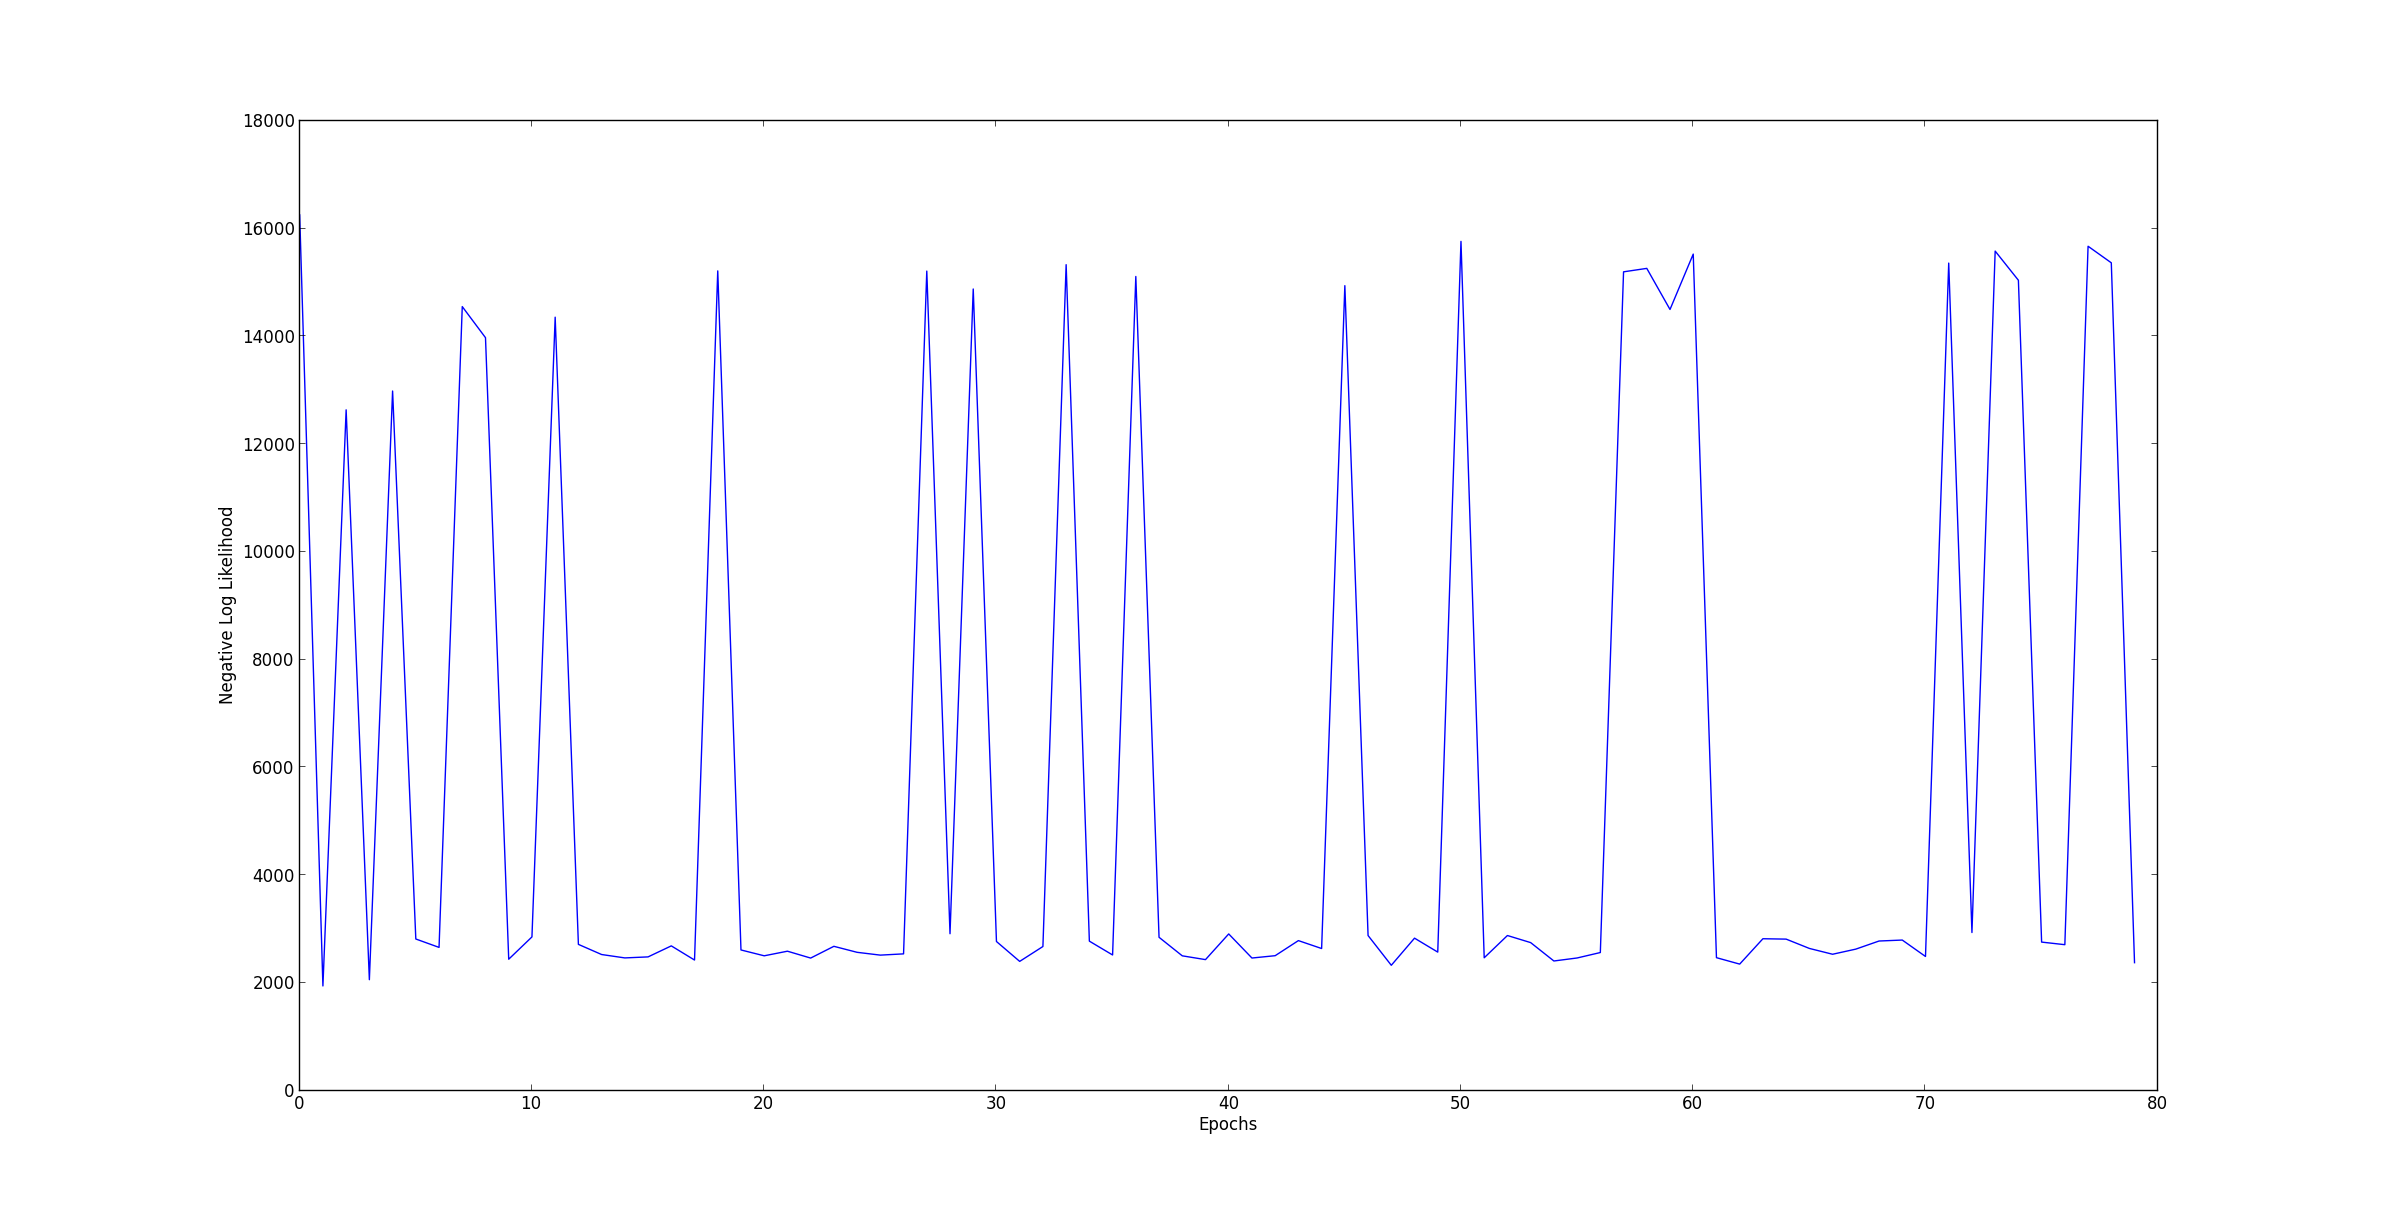
\includegraphics[width=10cm, height=8cm]{finalConnectedGraph}
  \caption{Objective function with straight line interpolation between points}
  \end{figure}
  \begin{figure}[H]
   \centering
  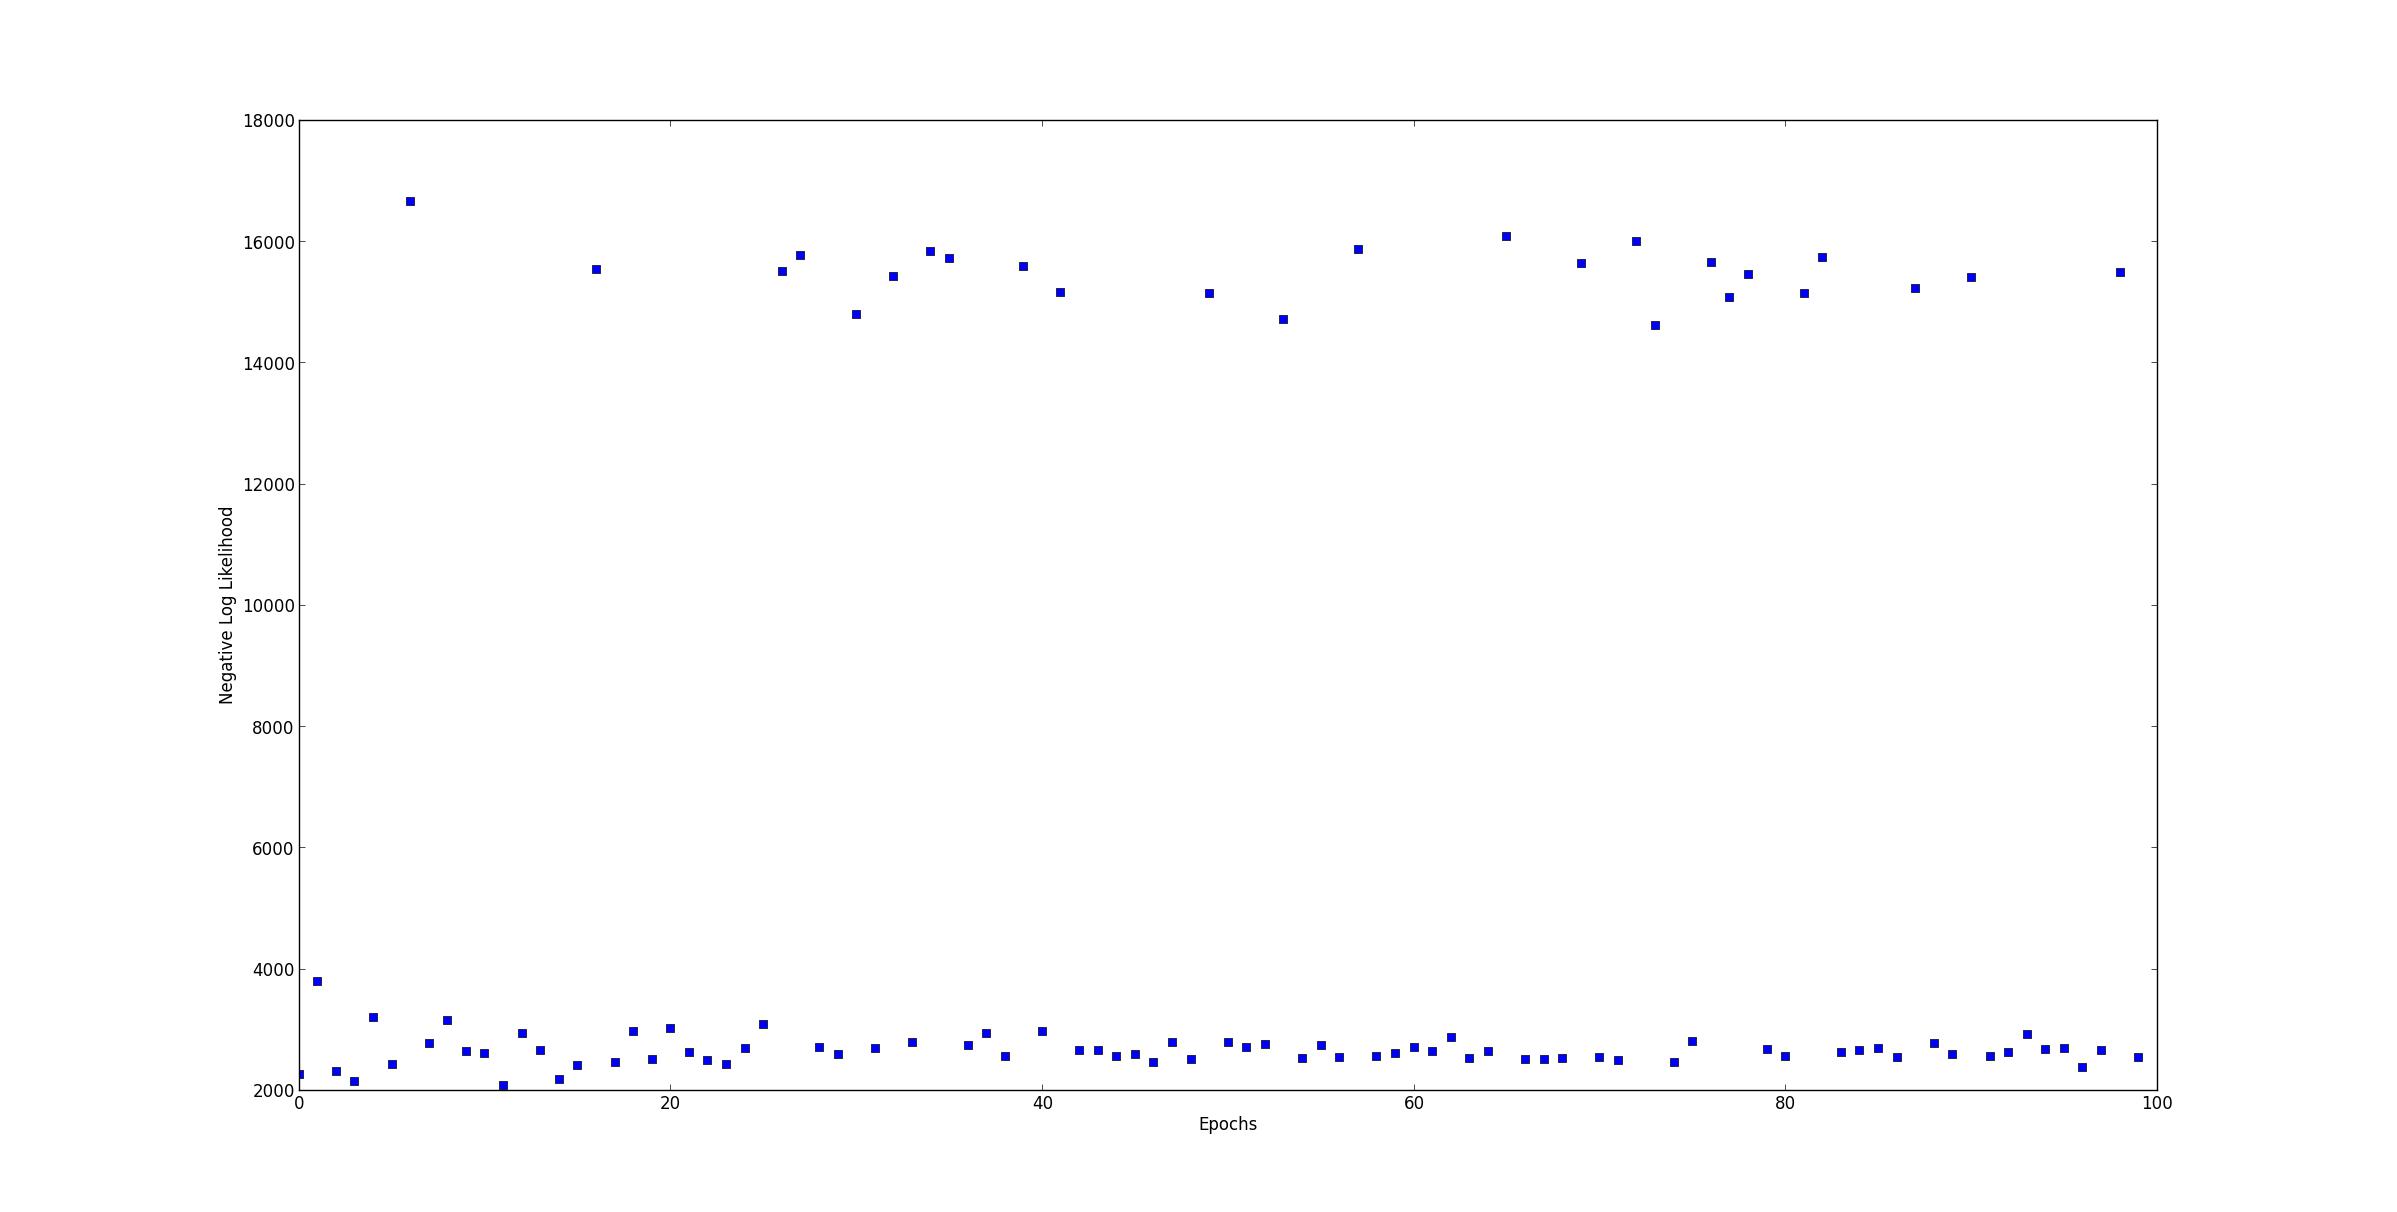
\includegraphics[width=10cm, height=8cm]{finalDotGraph}
  \caption{Objective function with straight line interpolation between points}
  \end{figure}
  \begin{figure}[H]
   \centering
  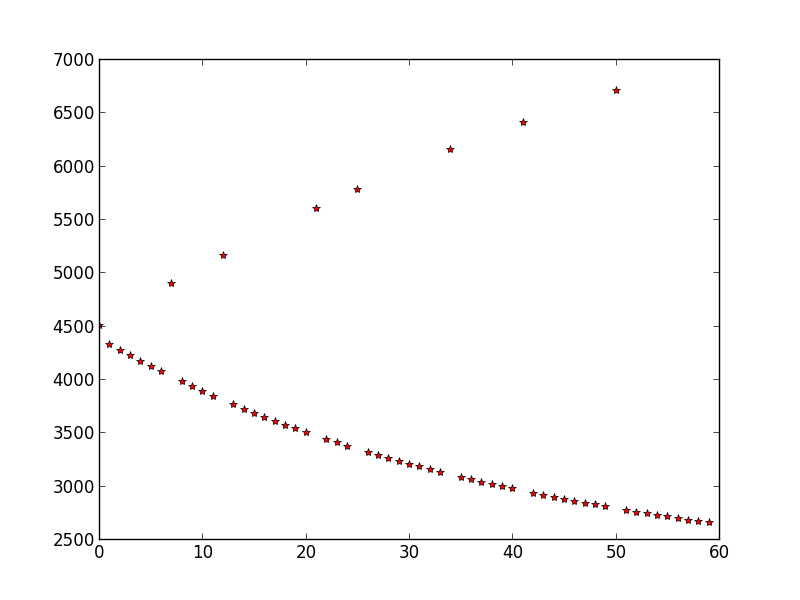
\includegraphics[width=10cm, height=8cm]{gd60}
  \caption{Objective function for gradient descent}
  \end{figure}
  
 Thats all for now!! Check out the code!! 

\end{document}
